\chapter{Implementation}
\label{ch:implementation}

This chapter describes how the system was built. Sections \ref{sec:projman} and \ref{sec:softengprac} present the software engineering tools and practices employed to aid the development process. Section \ref{sec:hardiss} explains the hardware problems that were encountered and how these were dealt with. Next, section \ref{sec:constread} goes through the steps taken to construct each reader node. Section \ref{sec:dataman} is concerned with how data was stored and managed in this system. Then, section \ref{sec:netcomm} describes how the reader nodes communicated RFID measurements over the network. Section \ref{sec:locest} explains how the methods for converting RSSI to distance and estimating the tag's location were implemented. Finally, section \ref{sec:webint} presents the web interface that was used to visualise the outputs of the system.

\section{Project management}
\label{sec:projman}

A number of considerations were taken into account when deciding how to manage this project. First, the system operates using a server-client model. This means that different software components are executing on multiple processing nodes. As a result, changes in one node need to be propagated in the whole system ensuring the consistency of the software.  Second, the software implementation is making use of different programming languages, multiple programming libraries, and a database management system. In order to ensure an iterative development process, where software components are constructed, debugged, and packaged together, it was decided to use the \textsc{Git} version control system\footnote{\textsc{Git} version control system - \url{http://git-scm.com/}}. This system keeps a distributed repository of all software and database files so that each node stores a copy of not only the whole software system, but also a complete history of changes. In addition, the use of a version control system stimulates the developer to merge a number of important changes into versions of the software. In this way, it becomes easy to track and monitor the project progress. The source code and documentation were hosted in a private repository on \textsc{GitHub}\footnote{The private project repository - \url{https://github.com/sandio/raspi-rfid-tracking}} with access granted to the people involved in developing and supervising the project.

\section{Software Engineering Practices}
\label{sec:softengprac}

A number of software engineering practices were of significant help when developing the RFID location sensing system. This section presents them and explains the problems that they solve.  

\subsection{Project decomposition}

It would have been a serious challenge to approach the project's task directly. The system consists of pieces of hardware that had to be orchestrated to solve a common problem. Therefore, it was very important to identify the system's components from early on. Hierarchical relationships between these parts were also defined. These steps ensured that the project could be divided into stages in order to systematically solve the main task. Regular deliveries of working components provided a more manageable way of constructing the final solution. For example, the work plan, devised before the start of the project, consisted of the following key activities:

\begin{enumerate}
 	\item Prepare the single-board computers
 	\item Construct functional RFID reader nodes
 	\item Receive information from the active RFID tag
 	\item Establish a network communication between nodes
 	\item Develop the localisation algorithm
 \end{enumerate}

Iterative construction of the system aided the development process. Problems and challenges were appearing gradually which helped solving them one at a time. 

\subsection{Object-oriented design}

This location sensing system is a combination of different software technologies. For instance, the system required an interface between a single-board computer and an RFID receiver. It also required means of communication between processing nodes. Logically, these and other requirements could be grouped into sets of functions, which is a motivation for employing an object-oriented design. This software methodology was used from the beginning of the project. Similar functionality is organised in a class. A class is responsible for all procedures concerning a particular part of the system. As a result, software is split into categories of functions, which makes it easy to address the class in charge of certain functionality.

Another benefit of the object-oriented design is modularity. For example, once input data is collected from all nodes it could be processed by a localisation algorithm in order to estimate the tag's position. Trilateration was chosen as the technique for computing locations. Object-oriented software development provides an easy way to experiment with different algorithms by substituting one class with another.

\subsection{System scalability}
\label{subsec:sysscal}

In this project, three single-board computers collaborate by exchanging RFID readings to localise a tagged object. Three reference points are needed in order to use trilateration in two dimensions  \cite{Zhang2009}. Nevertheless, more reader nodes could be used, in case multileration is implemented, to give a better approximation of a tag's position. Another scenario involves nodes disconnecting and later reappearing into the network. These possible cases show the dynamic nature of the system. It could scale up as the system grows, but also scale down if a reader node is faulty. This is an important property of the system, which was noted at the start of the project. To ensure scalability of the server-client model, the multi-threading programming model was used. It allows multiple threads to exist within the context of a single process. As a result, the system could concurrently receive RFID measurements from multiple reader nodes, update data structures, and compute the location of the unknown object.

% \subsection{Documentation}

% Writing documentation was an important part of this project. The source code of the system has been systematically documented throughout the development process. Using the inline comments specifying how the software components work, an Application Programming Interface (API) was constructed using \textsc{Sphinx}\footnote{\textsc{Sphinx} - a Python documentation generator - \url{http://sphinx-doc.org/index.html}}, a \textsc{Python} documentation generator. The API contains specifications of data structures, variables, and functions. It is a valuable source of information that provides a quick reference of how the system's components work and interact with each other. In addition, a manual for future users of the system was written. It gives a quick introduction of how to set up and use the system. The API and user manual can be viewed in Appendix \textbf{REF}  \textbf{TODO}.

% This project consists of both hardware and software components. In order to clearly understand how hardware components are connected and how software objects interact, a number of diagrams were used in Chapter \textbf{REF} and in the user manual. These diagrams were generated using \textsc{Blockdiag} \footnote{\textsc{Blockdiag} - simple diagram images generator - \url{http://blockdiag.com/en/}} , a diagram image generator written in \textsc{Python}.

\section{Hardware Issues}
\label{sec:hardiss}

This section describes two hardware problems that were identified while the project was running. It also explains how these were solved.

\subsection{Antenna Design}
\label{subsec:antdes}

When the hardware equipment for this project arrived, everything was in order except for the RFID tag. It was missing its antenna, which is a coiled wire. The antenna needed to have specific length ($2cm$) and width ($8mm$) of the coil. The tag was being detected by the RFID readers, but only in close range. Consequently, an antenna was required for the project to continue. A number of antennas were designed and soldered to the tag. Unfortunately, these were preventing the tag from being detected by the readers because they did not conform to the exact antenna specifications. The system could only receive measurements when these antennas were being touched by a human acting as an antenna extension. Another possible explanation was that the wires were composed of a bundle of smaller wire strings, which might have introduced interference in the radio transmission.

After a number of unsuccessful designs, an antenna was carefully constructed following the specifications of the manufacturer. Its wire was single and thick to ensure a strong signal would be emitted. Fortunately, this antenna worked perfectly and even increased the transmission range of the tag from eight meters as advertised by the manufacturer to 13 meters as identified during the hardware evaluation. The final antenna design can be seen on figure \ref{fig:tag}.

\subsection{Serial to USB converters}
\label{subsec:sertousb}

The RFID readers communicate their measurements using a RS-232 serial port. The authors of the SpotON localisation system have identified the limitations of such serial connections \cite[p. 6]{Hightower2000}. This type of cabling is not universal and has limited length. Moreover, RS-232 serial ports are neither present on the Raspberry Pi computers, nor on most modern computers. In order to provide a convenient way of communication between an RFID reader and a Raspberry Pi, serial to USB converters were ordered along with the readers.

A problem was detected during the initial serial communication experiments. When a serial connection is established, a flood of old identification and RSSI data filled the software input buffer of each Raspberry Pi. After in-depth research of the issue, there was a strong indication that this could be caused by the chip of the serial to USB converters. This chip was sending data with high speeds, although the tag transmits its identity every two and a half to three seconds. 

This unexpected behaviour needed further investigation. One of the converters was taken apart, as seen on figure \ref{fig:converter}. On the one hand, the sign on its case was indicating that it is model U-232-P9 manufactured by MCT Corp.. On the other hand, the chip model was PL2303HX detected by the Linux kernel as PL2303 manufactured by Prolific Technology, Inc.. Logically, one might ask what the brand of the converters was. In Linux, there is driver support for U-232-P9 as well. Attempts to use this driver instead of the automatically detected one resulted in a system crash. Further research indicated that this chip (PL2303HX) is an imitation of a genuine Prolific Technology chip \footnote{Prolific Technology Inc. PL2303 Windows Driver Download - \url{http://www.prolific.com.tw/US/ShowProduct.aspx?p_id=225&pcid=41}}. At this point, it was known that these converters were cheaper counterfeits. Nevertheless, they did work, but flooded the input buffers of the computers at the start of every serial connection.

\begin{figure}[h]
	\begin{center}
		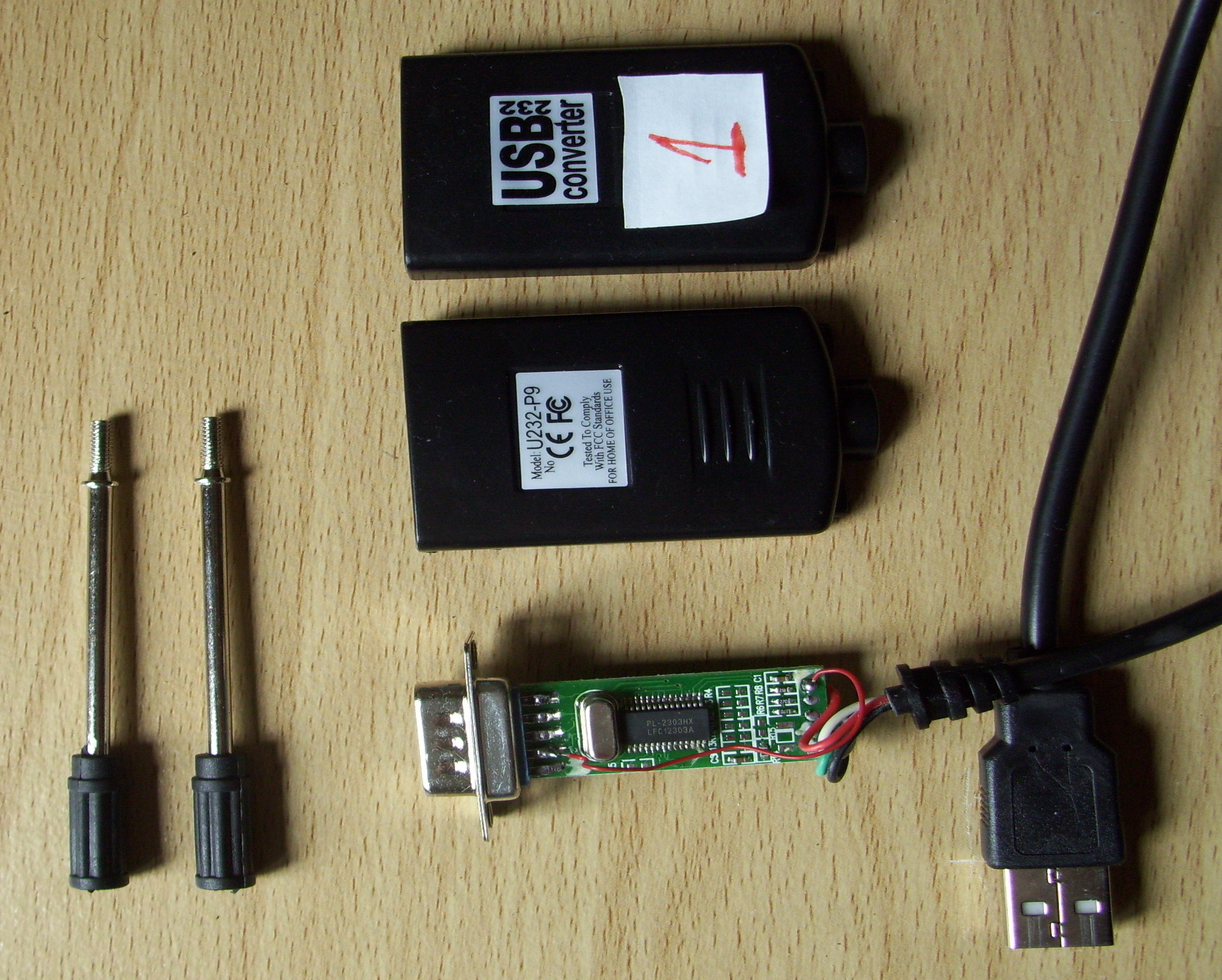
\includegraphics[width=.6\textwidth]{figures/converter2}
		\caption{The disassembled serial to USB converter.}
		\label{fig:converter}
	\end{center}
\end{figure}

The solution that worked best is to repeatedly drain the operating system input buffer until it holds a few bytes, an indication that the devices are communicating normally. A drawback of this approach is the time lost until the communication stabilises. Up to 58 initial buffer drains were recorded. A third of a second was chosen as a waiting time between buffer drains to ensure the operating system had time to perform this operation. This resulted in a maximum of 17.4 seconds ($58 \times 0.3s$) initial waiting time before the system could start its normal operation. In addition, each of the nodes had to not only wait between zero and a maximum time, but also ensure the other nodes had drained their buffers. This is because readings from all three nodes were needed for estimating the position of the tag. Due to the hardware nature of the problem, time would always be lost until different converters are tested.


\section{Reader nodes construction}
\label{sec:constread}

Constructing the reader nodes consisted of three main steps. First, an operating system had to be installed on each of the Raspberry Pi computers. The Raspbian Linux distribution\footnote{Raspbian Linux website - \url{http://www.raspbian.org/}} was selected because it is specifically optimised for these single-board computers and has a rich software base compiled for the ARM processor architecture. Second, the RFID readers and Raspberry Pi computers were connected through USB. Third, a software interface between the devices was implemented.

Most of the system was programmed in the \textsc{Python} programming language. All functions concerned with the serial communication of the devices were grouped together in a class called \textsf{SerialConnection}. The \textsc{pyserial} module was extensively used to implement the required functionality. The class consisted of methods for initialising a serial connection on a given port (\verb!/dev/ttyUSB0!), opening and closing this port for communication, flushing the input buffer, and reading incoming data. The last function had to be implemented to parse the information arriving from the readers. Most serial devices separate their individual readings by a newline character (\verb!\n!), carriage return (\verb!\r!), or a combination of both (\verb!\n\r!). These readers, however, separate measurements by a space character. As a result, \textsc{pyserial} functions for reading data could not be used. The solution implemented reads incoming information character by character until the separator is encountered. All methods provided by the \textsf{SerialConnection} class are illustrated as a sequence diagram on figure \ref{fig:seqserial}.

\begin{figure}[h]
	\begin{center}
		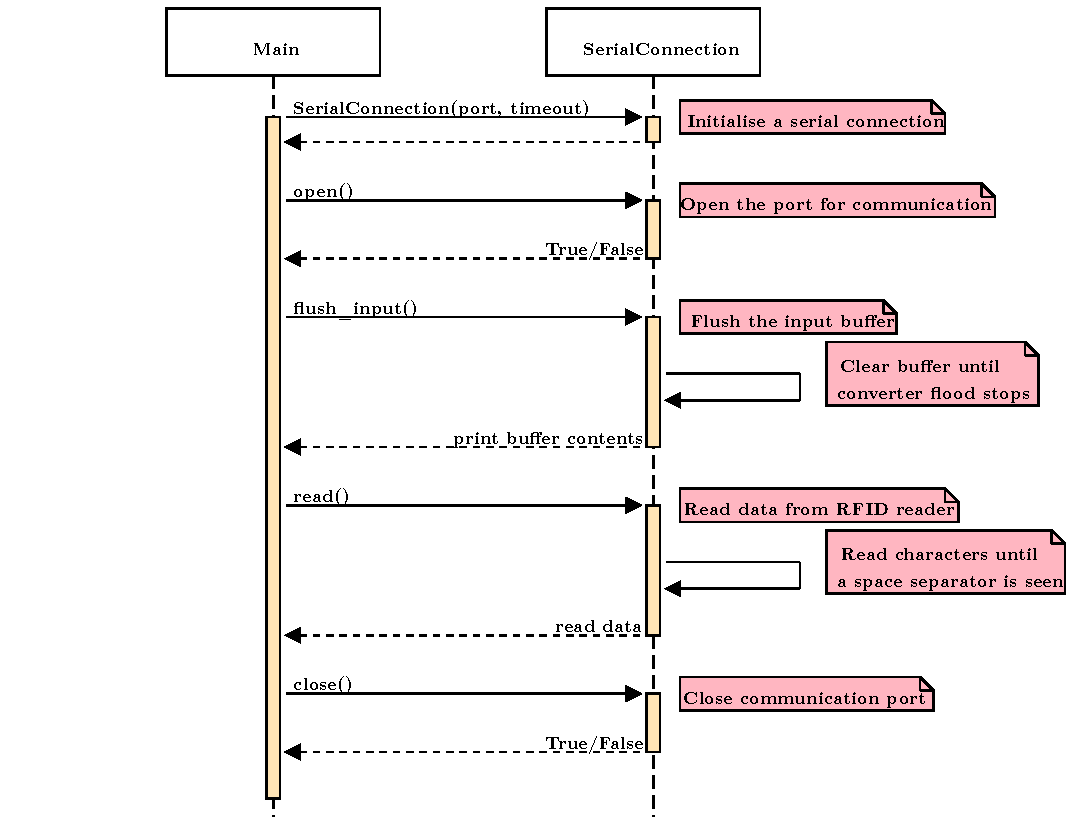
\includegraphics[width=1\textwidth]{figures/seqdiag/serial}
		\caption{A sequence diagram illustrating the methods of the \textsf{SerialConnection} class. The usual sequence in which they are called is shown from top to bottom.}
		\label{fig:seqserial}
	\end{center}
\end{figure}

\section{Data store and management}
\label{sec:dataman}

In this project, there were a number of important data fields that need to be accessed by processes and threads. For example, as discussed in section \ref{subsec:sysscal}, the system employed a server-client model where the server consisted of threads that simultaneously receive RFID readings from the other two nodes. These measurements needed to be stored, but also retrieved by the localisation algorithm or by the website visualiser, presented in section \ref{sec:webint}. This was a motivation for employing a data structure that was independent of the software components of the system. Support for simultaneous access of the data was also required.

The \textsc{SQLite}\footnote{\textsc{SQLite} website - \url{http://www.sqlite.org/}} database management system met the above requirements. It is a file-based system that operates without a server process, which spares system resources. \textsc{SQLite} serialises transactions so that all changes appear atomic and do not overlap in time. Database transactions might happen in parallel, but are processed in a sequential order by the database management system. Queries to the database were implemented in functions part of the \textsf{DatabaseHandler} class. Instances of this class were created in other classes where access to data was required.

Important data fields were the RFID readings, the positions of the reader nodes, and the estimated location of the RFID tag. These were stored in database tables. Examples of such data are shown in table \ref{tbl:sample}.

\begin{table}[h]
	\centering
	\begin{subtable}[b]{1\textwidth}
	\centering
	\begin{tabular}{|c|c|c|c|}
		\hline
		Reading & Node N\textsuperscript{\underline{o}} & Tag Id 	& RSSI	\\ \hline
		1		& 0										& 1Fwt		& 44	\\ \hline
		2		& 2										& 1Fwt		& 78	\\ \hline
		3		& 1										& 1Fwt		& 48	\\ \hline
		4		& 0										& 1Fwt		& 43	\\ \hline
	\end{tabular}
	\caption{Top four reader measurements.}
	\end{subtable}
	
	\begin{subtable}[b]{1\textwidth}
	\centering
	\begin{tabular}{|l|c|c|c|c|c|}
		\hline
		Node	& Node N\textsuperscript{\underline{o}} & $x$ 	& $y$ & $z$ & radius	\\ \hline
		Reader	& 0 									& 0.0 	& 3.0 & 0.0 & 4.0		\\ \hline
		Reader	& 1 									& 3.0 	& 0.0 & 0.0 & 0.786		\\ \hline
		Reader	& 2 									& 0.0 	& 0.0 & 0.0 & 5.0		\\ \hline
		Tag		& 3 									& 5.563 & 3.0 & 0.0 & 0.0		\\ \hline
	\end{tabular}
	\caption{Object positions in two dimensions.}
	\end{subtable}
	
	\caption{Sample data from the database of the system.}
	\label{tbl:sample}
\end{table}


\section{Network communication}
\label{sec:netcomm}

The overall software design of the system was introduced in section \ref{sec:softarch}. It defined the server-client model used to communicate RFID readings over a computer network. This section is concerned with detailing how this network communication was implemented.

Two of the Raspberry Pi computers acted as nodes that gathered information from their RFID readers to immediately send it over the network to the third node. This node was designated as the server of the system collecting readings and using this information to compute the tag's position. The network communication was implemented using socket programming. Python's \textsc{socket} module offered all required functions.

At the client side, the \textsf{NetworkClient} class was responsible for initialising a client streaming socket. A client uses a client socket to connect to a server socket. A streaming socket was chosen because nodes communicate a continuous stream of data to the server node. After this socket is created, a connection request is sent to a server socket specifying the network address and port of the server computer.

At the server side, the \textsf{NetworkServer} class creates a server streaming socket. Next, this socket is bound to the network address of the machine on a specified port. Then, the server socket starts listening for incoming connections. The server checks for connection requests using a non-blocking approach. This means that the programme tests if a request is available without indefinitely waiting for one to arrive, thus being able to terminate if requested. Once a client tries to connect, the \textsf{NetworkServer} accepts it by creating a client socket at the server side. At this point the only thing left to serve the incoming request is for the server to spawn a thread that handles the connection from this moment on. The motivation for using a threaded network server is discussed in section \ref{subsec:sysscal}.

Each network server thread receives incoming data from one client node. Listening on the socket for new information is again implemented using a non-blocking socket. If the receive buffer is empty, the receiver thread will not block indefinitely until data arrive. Rather, this buffer is checked constantly, but the thread could still be controlled by its parent process. If new data is available, it is read and inserted into the database using an instance of the \textsf{DatabaseHandler} class.

In case the system is interrupted by the user, the network server sends a stop signal to each of its threads and waits for them to terminate individually before terminating itself. This is the behaviour of the \textsc{join(timeout)} function of the Python's \textsf{threading} module. All the functionality described above is illustrated as a sequence diagram on figure
\ref{fig:seqnet}.

\begin{figure}[h]
	\begin{center}
		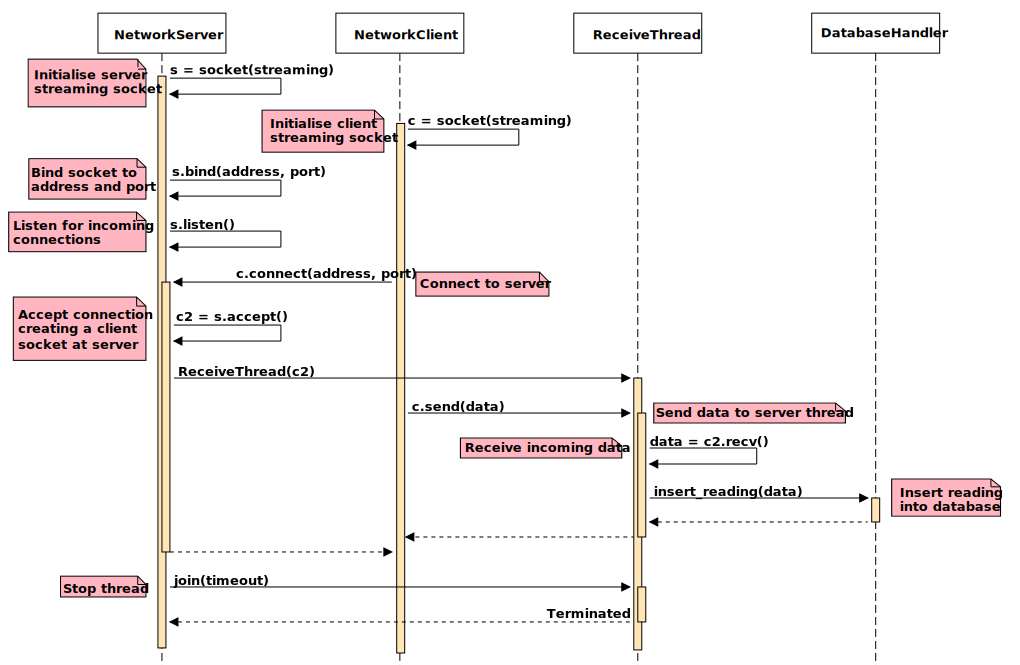
\includegraphics[width=1\textwidth]{figures/seqdiag/network}
		\caption{A sequence diagram illustrating the methods of the \textsf{NetworkServer}, \textsf{NetworkClient}, and \textsf{ReceiveThread} classes. The usual sequence in which they are called is shown from top to bottom.}
		\label{fig:seqnet}
	\end{center}
\end{figure}

\section{Location estimation}
\label{sec:locest}

This section presents the implementation details of converting RSSI to distance and computing the unknown position of the RFID tag using the trilateration technique.

\subsection{RSSI to distance conversion}

The implementation of converting RSSI to distance relied on the methodology described in section \ref{subsec:transtbl}. More specifically, the programme uses an instance of the \textsf{DatabaseHandler} class to get the three most recent RFID readings from the database. For each of these, an RSSI value is converted to distance in meters based on the translation table of the reader at which the measurement was recorded. This is needed because of the slight hardware differences between the RFID readers. Next, an integer factor is added to an RSSI value to account for the battery power drop as it is being used. Then, the position of an RSSI measurement in the translation table is determined. Finally, RSSI is linearly converted to distance for the specific range.

\subsection{Trilateration}
\label{subsec:trilatimpl}

The trilateration position estimation technique was implemented relying on the general three-dimensional solution of the method presented in section \ref{sec:trilatmeth}. The algorithm accepts as inputs the positions of the three reader nodes and their RSSI measurements. The positions are fetched from the database and the RSSI values are converted to distance using the aforementioned steps. All equations of the trilateration method were directly implemented with the aid of the \textsc{math} (mathematical functions) and \textsc{numpy} (scientific computing) modules. It was noted that a number of recurring intermediate computations could be computed once and inserted in the equations as variables. Such computations included $\vec p_2 - \vec p_1$, $\vec p_3 - \vec p_1$, and $\hat e_x i$. The algorithm outputs the estimated location of the unknown object. This result is inserted into the database so that it could be visualised on the web interface. Figure \ref{fig:seqtrilat} is a sequence diagram showing the functions of the localisation algorithm and how it interacts with other software components. 

\begin{figure}[h]
	\begin{center}
		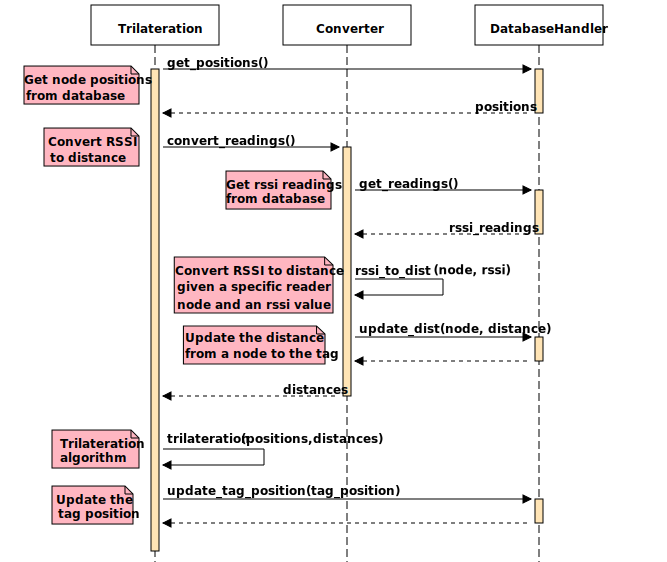
\includegraphics[width=1\textwidth]{figures/seqdiag/trilat}
		\caption{A sequence diagram illustrating the methods of the \textsf{Trilateration} class. The usual sequence in which they are called is shown from top to bottom.}
		\label{fig:seqtrilat}
	\end{center}
\end{figure}

\section{Web Interface}
\label{sec:webint}

The web interface is a website that runs on the server node. It main purpose is to provide a convenient interface to interact with the system. The web page is automatically refreshed every three seconds, which is roughly the interval at which the RFID tag transmits its identity. The website provides the following information:

\begin{itemize}
	\item the positions of the readers and tag,
	\item a form to change the positions of the reader nodes,
	\item the error in meters of the estimated position to the true one,
	\item a graph with reader positions and their distance from the tag,
	\item a table with the three most recent RFID readings,
	\item a table providing status information about the Raspberry Pis. 
\end{itemize}

The website is implemented in the \textsc{PHP} programming language. All information is provided from the \textsc{SQLite} database. The website runs on an \textsc{Apache} HTTP web server installed on the server node. The website was password protected to allow only people involved in this project to access it through the Internet. Figure \ref{fig:web} is screen capture of the web interface.

\begin{figure}[h]
	\begin{center}
		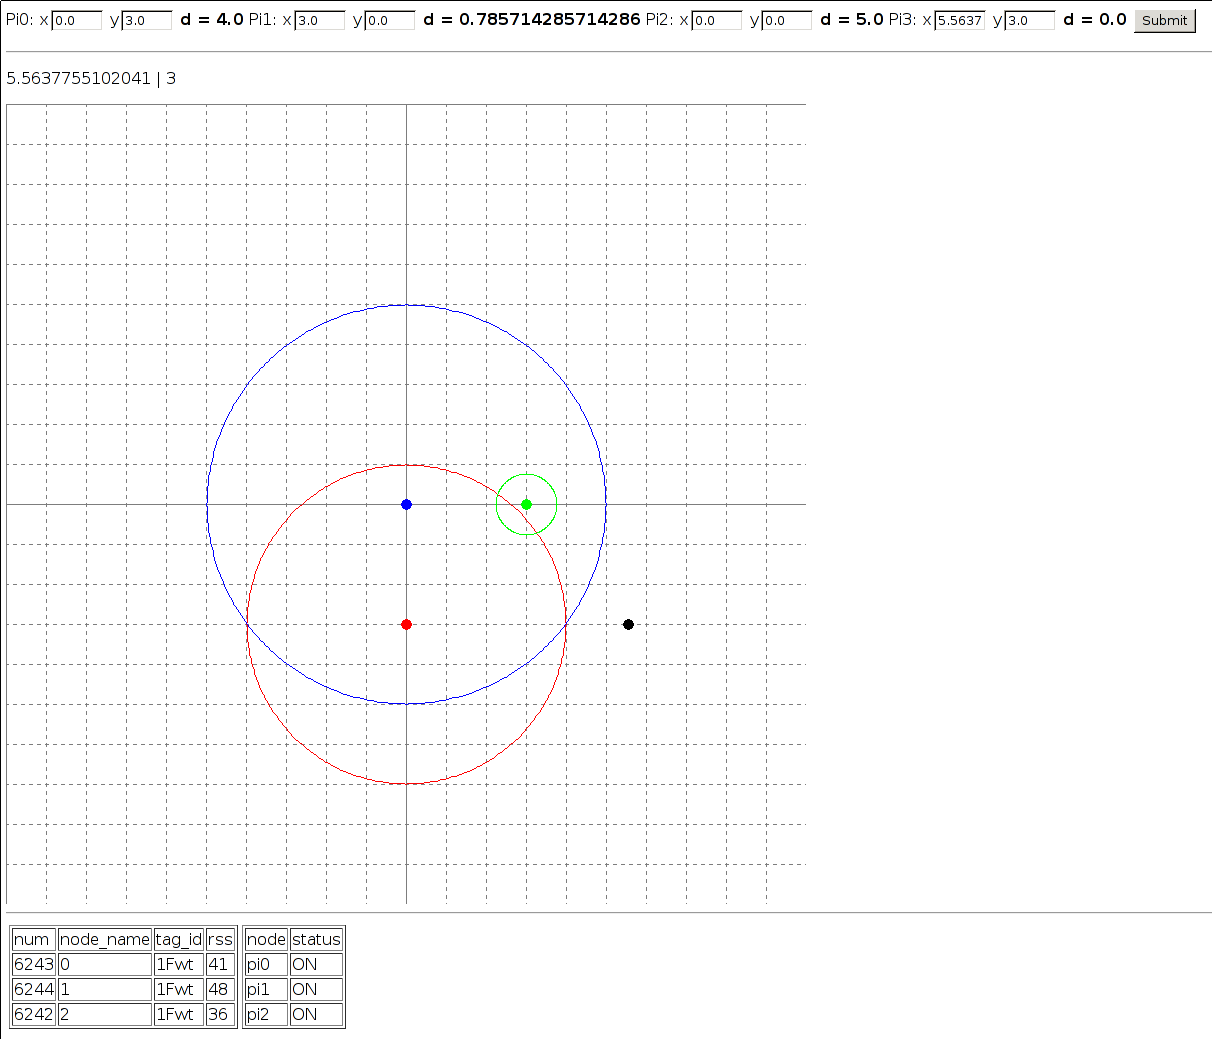
\includegraphics[width=.8\textwidth]{figures/sim}
		\caption{The web interface running on the server node.}
		\label{fig:web}
	\end{center}
\end{figure}

\begin{figure}[h]
	\begin{center}
		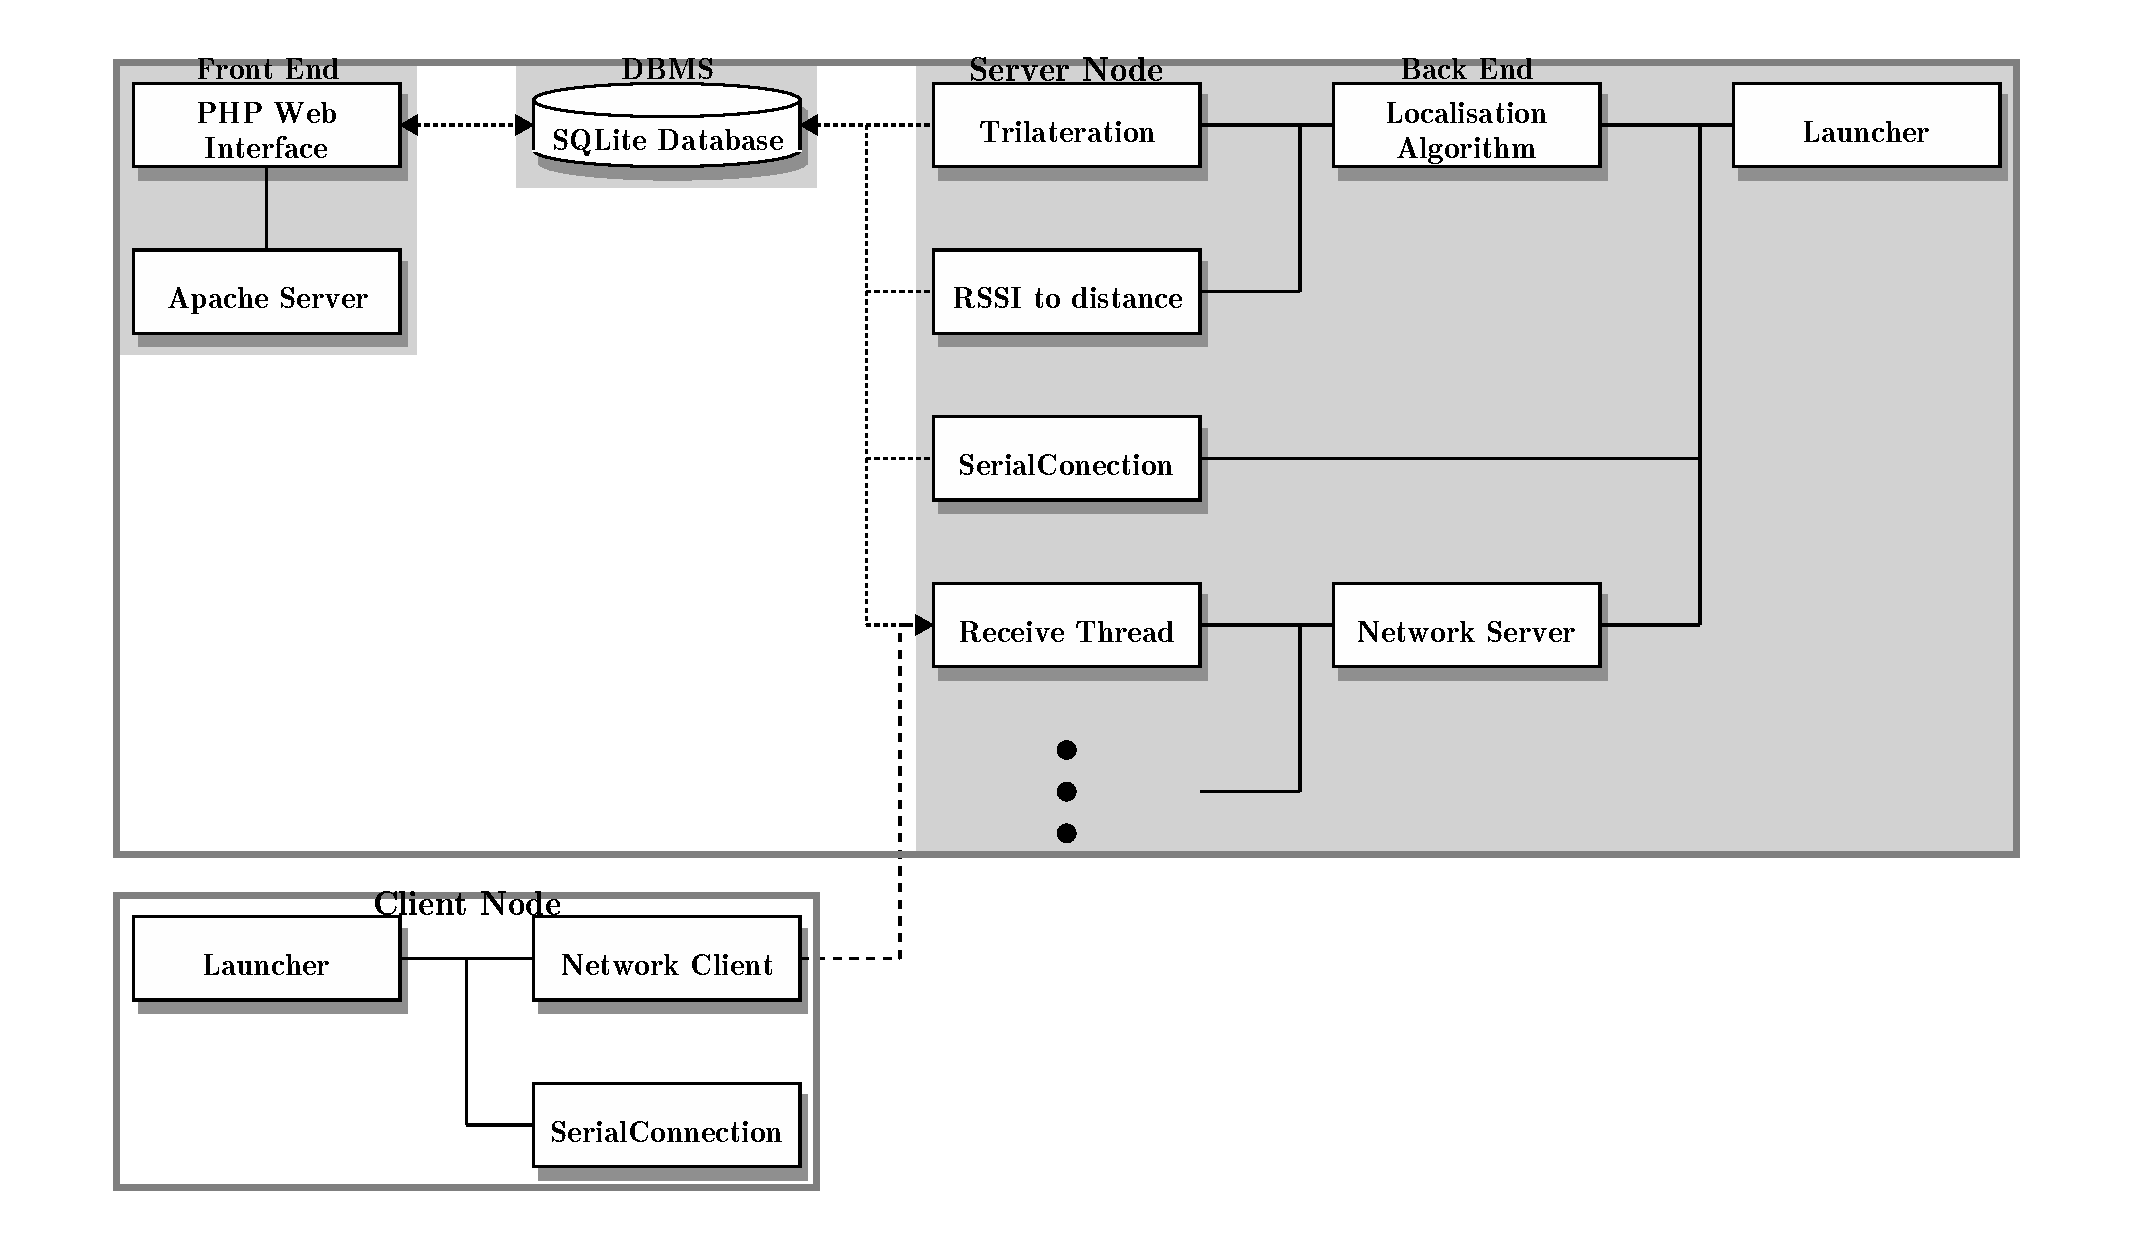
\includegraphics[width=1\textwidth]{figures/blockdiag/system}
		\caption{A diagram illustrating all software components of the system. Both server and client nodes are shown.}
		\label{fig:sys}
	\end{center}
\end{figure}

\section{Summary}

This chapter detailed the software practices that helped develop this system. It also described hardware issues that were faced throughout the project. Next, implementation details of all parts of the system were presented. Figure \ref{fig:sys} is a diagram of all system components. The next chapter discusses the evaluation of the system's hardware component and the overall system's performance in terms of localisation accuracy.
